\documentclass{article}
\usepackage{amsmath}
\usepackage{graphicx}
\usepackage{subcaption}
\usepackage[slovene]{babel}

\newtheorem{definicija}{Definicija}

\title{Parametrizirana kompleksnost koordiniranega načrtovanja gibanja}

\begin{document}

Dana je mreža $G$ velikosti $n \times m$ in $k$ robotov, opisanih s pari točk $\mathcal{R} = \{ (s_i, t_i) | i \in [ k ] \} $, kjer prva komponenta $s_i$ predstavlja začetno lego robota $i$, $t_i$ pa njegovo končno točko. Roboti se lahko premikajo v sosednja polja ali pa ostanejo na mestu, dokler ne trčijo z drugim robotom. Pot robota $i$ je definirana kot nabor $W_i = (u_0 \dots u_t)$, kjer je $u_0 = s_i$, $u_t = t_i$, in za vsak $j \in [t]$ velja $u_{j-1} = u_j$ ali $u_{j-1} u_j \in E(G)$. Cilj je oblikovati urnik premikanja robotov od začetnih do končnih točk, pri čemer problem imenujemo CMP-M, če želimo, da roboti dosežejo svoje destinacije v največ $l$ časovnih korakih, in CMP-L, če je cilj najti urnik, kjer je skupna pot robotov manjša od $\lambda$.

\begin{figure}[h]
    \centering
    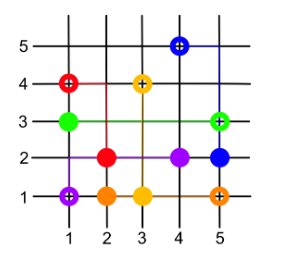
\includegraphics[width=4cm]{cmp-m.png}
    \caption{Rešen CMP-M problem s šestimi roboti in štirimi časovnimi koraki.}
\end{figure}

V članku sta problema CMP-M in CMP-L parametrizirana s številom robotov $k$. Oba problema sta traktabilna s fiksnim parametrom (FPT), kar pomeni, da lahko rezultat najdemo v času $f(k) \cdot n^{O(1)}$, kjer je $f$ funkcija, in $n$ velikost vhoda.

Dokaz, da je CMP-M FTP, je sestavljen iz dveh korakov. Najprej se pokaže, da ima vsak rešljiv problem rešitev, katere število zavojev je omejeno s funkcijo parametra $k$. Pri izpeljavi se definira \textbf{slack}$_T (R_i)$, ki meri število zapravljenih časovnih korakov med premikom robota na nekem podintervalu. Tako se ločijo roboti na tiste z majhnim in tiste z velikim \textbf{slack}om, število zavojev robotov obeh skupin pa je navzgor omejeno. 
% Dokaz, da je CMP-M FTP, je sestavljen iz dveh korakov. Najprej pokažemo, da ima vsak rešljiv problem kanonično rešitev, katere število zavojev je omejeno s funkcijo parametra $k$. Pri izpeljavi definiramo \textbf{slack}$_T (R_i)$, % = (t_2 - t_1) - \Delta (u_p, u_q)$, 
% ki meri število zapravljenih časovnih korakov med premikom robota na nekem podintervalu. %od $u_p$ do $u_q$ v odvisnosti od Manhatannove razdalje $\Delta$. 
% Tako ločimo robote na tiste z majhnim in tiste z velikim \textbf{slack}om, in pokažemo njihovo strogo ločitev na časovnem intervalu, ki ga imenujemo dober interval.
% \begin{definicija}
% Za funkcije $\sigma (k), \gamma (k)$ in $d(k)$, kjer $\sigma (k) < \gamma (k)$, je interval $T \subset [0, l]$ \emph{$[\sigma, \gamma]$-dober interval} glede na $d(k)$, če lahko množico $R$ razdelimo na $R_S$ in $R_L$ tako, da za vsak $R \in R_S$ in za vsak $R' \in R_L$ velja:
% \begin{itemize}
% \item \textbf{slack}$_T (R) \leq \sigma (k)$ in \textbf{slack}$_T (R') \geq \gamma (k)$,
% \item $\Delta_t (R, R') \geq d(k)$,
% \item obstaja robot v $R_L$, katerega število zavojev je večje od $3 k^k (\sigma (k) + 1) + \sigma (k)$.
% \end{itemize}
% \end{definicija}
V drugem delu se pokaže obstoj rešitve z razdelitvijo problema na več posnetkov mreže. Za vsak posnetek konstruiramo ekvivalenten problem v linearnem programiranju in preverimo, ali je slednji rešljiv v času FPT. V kolikor je, je CMP-M rešljiv v času FPT.
Podobno se dokaže, da je problem CMP-L, ki je parametriziran s številom robotov, rešljiv v času FPT. % Namesto dobrega intervala se definira dober pravokotnik, ki je opredeljen z diagonalno nasprotnima vozliščema $u_i$ in $u_j$.

% \begin{definicija}
% Naj bo $W$ del poti robota $R$ na časovnem intervalu $T$, tako da je zaporedje zavojev $M$, ki pripada poti $W$, monotono, tj. smeri zavojev se izmenjujejo v dveh smereh. \textbf{Pravokotnik $(M)$} je \emph{dober} glede na funkcijo $\sigma (k)$ in $T' \subset T$, če veljajo naslednje lastnosti:
% \begin{itemize}
% \item Množica robotov v pravokotniku se ohranja med celim $T'$.
% \item Za vsak $R \in R$ velja \textbf{slack}$_{T'} (R) \geq \sigma (k)$.
% \item Vsak robot se premika v smeri $M$.
% \item Število zavojev vsakega robota na pravokotniku je vsaj $\sigma (k)$.
% \end{itemize}
% \end{definicija}

V članku je problem CMP parametriziran tudi s ciljem, ki ga želimo optimizirati. Tako lahko CMP-L parametriziramo s skupno dolžino poti vseh robotov. Z izčrpnim razvejitvenim algoritmom ugotovimo, da je problem rešljiv v času FPT.

Če parametriziramo CMP-M glede na število časovnih korakov, se soočamo z NP-težkim problemom, kar dokažemo z redukcijo na NP-težek problem 4-omejenega ravninskega 3-SAT, kjer je potrebno evaluirati CNF formulo na ravninskem grafu. Ta problem prevedemo v situacijo, kjer imamo dani graf in množico parov vozlišč ter moramo ugotoviti, ali obstaja množica disjunktnih poti, ki bi povezala vsak par danih vozlišč s potjo dolžine največ $d$. Pri redukciji slednjega problema do CMP-M uporabimo nekaj pomožnih definicij, natančneje tok in puščico robotov, ki usmerjata glavne robote.
\begin{figure}[h]
    \centering
    \begin{subfigure}{0.65\textwidth}
      \centering
      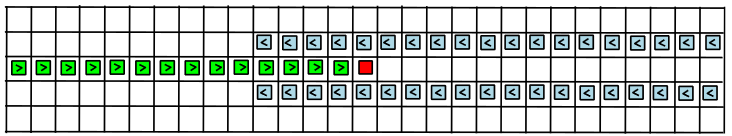
\includegraphics[width=\linewidth]{tok.png}
      \caption{Tok robotov.}
    \end{subfigure}\hfill
    \begin{subfigure}{0.25\textwidth}
      \centering
      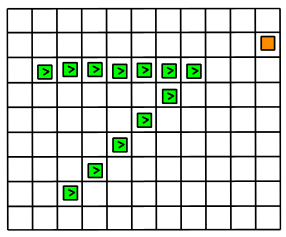
\includegraphics[width=\linewidth]{puscica.png}
      \caption{Puščica robotov}
    \end{subfigure}
    \end{figure}

Posledično je CMP-M, parametriziran s skupno dolžino poti robotov, NP-težek problem, saj ga je mogoče reducirati iz 4-omejenega ravninskega 3-SAT problema. Avtorji upajo, da bo ta dokaz NP-težkosti služil kot osnova za dokaze NP-težkosti drugih geometrijskih in topoloških problemov.
\end{document}